\documentclass{article}

\usepackage{mathrsfs,amsmath}
\usepackage{xcolor}
\usepackage{titlesec}
\usepackage{listings}
\usepackage{syntax}
\usepackage{pythonhighlighting}
\usepackage{graphicx}

\graphicspath{ {./assets/} }

\usepackage[margin=1.4in]{geometry}

\title{Handout \#10 | CS 471} 
\author{Jared Dyreson\\ 
        California State University, Fullerton}

\DeclareRobustCommand{\bowtie}{%
  \mathrel\triangleright\joinrel\mathrel\triangleleft}


\usepackage [english]{babel}
\usepackage [autostyle, english = american]{csquotes}
\MakeOuterQuote{"}

\titlespacing*{\section}
{0pt}{5.5ex plus 1ex minus .2ex}{4.3ex plus .2ex}
\titlespacing*{\subsection}
{0pt}{5.5ex plus 1ex minus .2ex}{4.3ex plus .2ex}

\usepackage{hyperref}
\hypersetup{
    colorlinks,
    citecolor=black,
    filecolor=black,
    linkcolor=black,
    urlcolor=black
}

\begin{document}

\maketitle
\tableofcontents

\newpage

\section{Questions}

\begin{enumerate}
\item \textcolor{red}{What are the advantages of web caching in terms of:}

\begin{itemize}
\item Improving response time:
\item Reducing congestion of the access link:
\item Filtering traffic:
\end{itemize}

\item Give an example of illustrating how conditional GET works

\begin{itemize}
\item We can visit a website, which will allow us to save the HTML page to disk. After doing some other browsing, we can revisit the same page indicating we only want the page if it has changed since we last obtained it. If it does not meet this criteria, we will just load from disk.
\end{itemize}

\item There are 33 users on the network. Each user requests web objects at a rate of 30 objects per-second. Suppose each object is 1000 bits long, the LAN connection is 100 MBPs, and the access link connecting the LAN to the outside is 1 MBPs. What is the:

\begin{itemize}
\item \textbf{Utilization of the LAN link:} 33 users all connected on a 100 MBPs link $\implies$ 3 MBPs link.
\item \textbf{Utilization of the access link:} If all 33 users attempted to access 30 objects all at the same time, then it would $33 \times 30 = 990 \text{ kbps }$
\item This is less than the LAN connection to the outside web, therefore no slow down
\end{itemize}

\item A system resides on the LAN. A web cache server resides on the same LAN. The cache hit rate is 20\%. It takes 4 seconds and 2 seconds to retrieve an object from the origin web server and web cache respectively. What will the average required for fetching the object?

\begin{itemize}
\item $0.2 \times 2 + 0.8 \times (2 + 4) = 5.2 \text{ seconds }$
\end{itemize}
\newpage

\item What is Squid (in relation to web caching)?

\begin{figure}[!h]
\centering
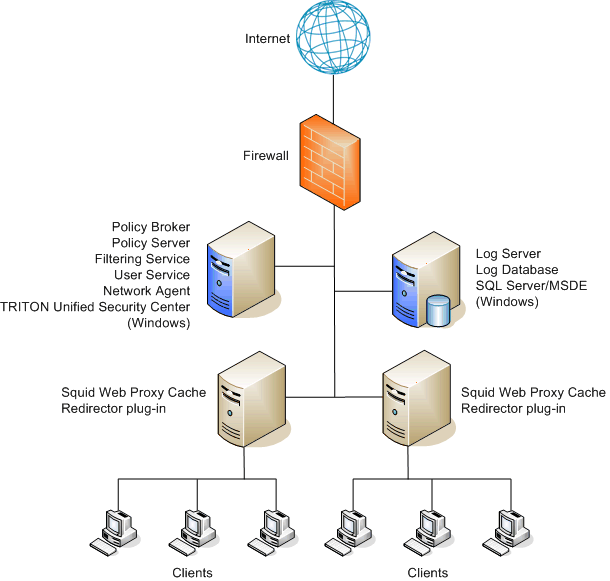
\includegraphics[width=8cm]{Squid_Array2}
\end{figure}

\begin{itemize}
\item A caching proxy for the Web supporting HTTP, HTTPS, FTP, and more. It reduces bandwidth and improves response times by caching and reusing frequently-requested web pages
\item More information can be accessed \href{http://www.squid-cache.org/}{\underline{here}}.
\end{itemize}

\item Nowadays more and more webpages are becoming dynamic (being formulated by a web server such as Flask). How will this affect web caching?

\begin{itemize}
\item Dynamic web pages are often cached when there are few or no changes expected and the page is anticipated to receive considerable amount of web traffic that would wastefully strain the server and slow down page loading if it had to generate the pages on the fly for each request. 
\item An example of dynamic pages can be found \href{https://github.com/JaredDyreson/personal-website/blob/master/personalwebsite/templates/demos.html}{\underline{here}}. My website uses Flask as the back end to dish out dynamic pages.
\end{itemize}
\end{enumerate}

\end{document}

